\chapter{Researching homogeneous temporal periods}\label{chp:3}

\minitoc

\clearpage

Although the recommendations for the use of the substances are formulated in the marketing authorization issued by ANSES \cite{ephy}, their practical use is not subject to control by the agency. Cultivation practises depend on meteorological conditions and professional habits. This partly explains the spatiotemporal heterogeneity. Our goal is to find homogeneous time periods and geographic areas and make a statistical comparison of these regions in these stable time periods to support the expert analysis. In this chapter, we focus on identifying stable temporal patterns using change point detection methods. This mathematical area is covered by several surveys \cite{truong2020,basseville1993detection}. We have focused on methods that seem appropriate for the application domain of phytopharmacovigilance. For example, this work will focus only on the offline methods that we will develop in the following sections. This choice was motivated by the speed of data collection and storage of pesticide concentrations data. Nevertheless, for readers who wish to refer to it, we can state that there is no shortage of online detection methods in the literature \cite{liu2017change,Li2021,hohle2010online,ranganathan2010pliss,li2015m}.

\section{Model and cost functions}\label{chp:3:1}

We describe the most general configuration of a change-point model appropriate for concentration data. We consider a signal consisting of observations $\bm y = (y_1,...,y_n)$, which are the realisations of random variables $Y_1,...,Y_n$. The variables $Y_i$ are recorded sequentially, and the recording times are not necessarily equidistant. Thus, the indices in $Y_i$ are only indicators of the order of occurrence in the sample and not of the observation times. Some properties (trend, mean, variance, etc...) of the signal $\bm y$ are supposed to change at the $K^*$ times points $\tau^*_1 <... < \tau^*_k <... < \tau^*_{K^*}$. We use the following convention, let $\tau^*_0 = 0$ and $\tau^*_{K^*+1} = n$. The purpose of breakpoint detection is to estimate the positions $\tau^*_k$ and the number of breaks $K^*$ when they are unknown. The goal is to identify the data segments in which these properties are stable. We denote $y_{u:v}$ as a segment of the signal from the u-th coordinate to the v-th. \\
According to the nomenclature proposed by \cite{truong2020}, change point detection methods operate on a cost function $W$. This function associates a cost to the segment it is evaluated on. Intuitively, the more properties (on which changes are investigated) of the segment $y_{u:v}$ are homogeneous, the lower the cost $W(y_{u:v})$ is. We define, for any $y_{u:v}$, $\TT = \{\tau_1,\dots,\tau_K\} \subset \{u,\dots,v\}$ a set of ordered indices and $\lvert \TT \rvert$ its cardinal. Implicitly, we define $\tau_0 = u$ and $\tau_{K+1} = v$. Although this notation is often used for the full signal $\bm y$, we will always indicate the data segment from which $\TT$ is drawn in the parameters of the functions using the notation $\TT$. The total cost $\CC(\bm y,\TT)$ associated with a segmentation defined by $\TT$ is given as the sum of the costs of all segments:

\begin{equation}\label{chp:3:costfunc}
\CC(\bm y,\TT) = \sum_{k=0}^{\lvert \TT \rvert} W(y_{\tau_k+1:\tau_{k+1}}), 
\end{equation}     

With these notations and the knowledge of the number of change points $K^*$ that occurred in $\bm y$, the change point problem can be posed as an optimization problem:

\begin{equation}\label{chp:3:optKknown}
 \widehat{\TT}  = \arg \min_{\lvert \TT \rvert = K^*}  \CC(\bm y, \TT) = \arg \min_{\lvert \TT \rvert = K^*} \sum_{k=0}^{K^*} W(y_{\tau_k+1:\tau_{k+1}})   
\end{equation}

The choice of cost function determines the type of changes (in trend, mean, etc.) targeted by the detection. Figure \ref{fig:ex_cp} illustrates two different types of changes that may be of interest for change point detection. In the next parts of this section, we distinguish the cost functions according to the statistical inferences on which they are based. We give a non-exhaustive list of cost functions for each inference.

\begin{figure}[ht]
    \centering
    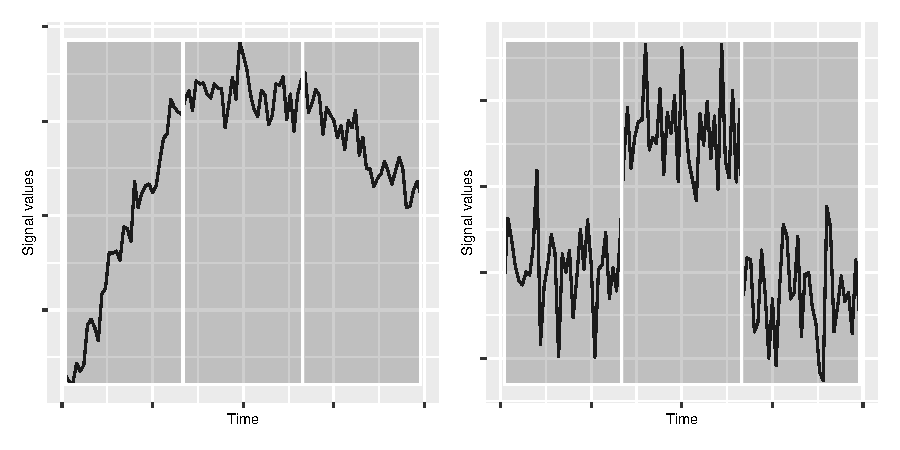
\includegraphics{figs/Chap2/Ex_CP_cost.pdf}
    \caption{Examples of types of change point detection. The figure on the left illustrates changes in trend whereas the figure on the right illustrates changes in mean.}
    \label{fig:ex_cp}
\end{figure}

\subsection{Parametric inference}

In the parametric case, the detection depends heavily on what we are looking for in the signal $\bm y$. For example, searching for slope changes in a signal \cite{Bai1994,Fearnhead2018} does not require the same modelling as detecting changes in the mean \cite{Frick2014,chen2012parametric}. 

A first classical cost function is based on the maximum likelihood estimation. In this setting, the observations located in the $k$-th segment is supposed to be following a distribution $Q$ depending on a vector of parameters $\theta^*_k$ with $\theta_k \in \Theta$ being a compact subset of $\mathbb{R}^p$. More formally, we have that:
$$y_t \sim f(.;\theta^*_k)\mathbbm{1}_{\tau^*_{k}+1\leq t \leq \tau^*_{k+1}},$$
with $f$ being the density function of distribution $Q$. In other words, we suppose that all observations emanate from the same distribution $Q$ but the values of $\theta^*_k$ change abruptly at each change-point $\tau^*_k$. The cost function used to evaluate segments in this context is the negative log-likelihood. Hence, for a segment $y_{u:v}$ with $u < v$, we can write:  
$$W(y_{u:v}) = -\sup_{\bm \theta \in \Theta} \sum_{i = u}^{v} \ln f(y_i; \bm \theta)$$
This method would prove useful in the example presented in the right side of Figure \ref{fig:ex_cp}. Applying the maximum likelihood estimator on the mean of Gaussian distribution would provide satisfying results. Other distributions than the Gaussian were investigated since it is not always well suited for data (especially concentrations data),  

Cost functions adapted for changes in trend rely on piecewise linear regression. We place ourselves in the simpliest case where $\bm y$ is univariate response to observed covariates $\{x_t\}_{t=1}^n$ such that $x_t \in \mathbb{R}^p$. Observations located in the $k$-th segment is supposed can be written as:   
$$y_t \sim (x'_t\theta^*_k + \epsilon_t)\mathbbm{1}_{\tau^*_{k}+1\leq t \leq \tau^*_{k+1}},$$
where $\theta^*_k \in \mathbb{R}^p$ are the regression parameters and $\epsilon_t$ is the noise of the signal. The adapted cost function in this configuration uses the least squares estimation and is expressed as:
$$W(y_{u:v}) = \min_{\theta \in \mathbb{R}^p}\sum_{t=u+1}^v(y_t-x'_t\theta)^2$$ 
This modeling is perfectly suited for the detection of the changes in the left example of Figure \ref{fig:ex_cp}. 



\subsection{Non-parametric inference}

The cost function for a segment can also be adapted for nonparametric statistical inference. Several strategies have been developed in the literature over time. These include the nonparametric maximum likelihood method \cite{Zou2014,Einmahl2003}, kernel methods \cite{Harchaoui2008,li2015m}, and rank-based methods \cite{Pettitt1980,Wang2019}. We will focus on the latter because it was adapted for censored observations in \cite{lung2015}.  

Detecting a breakpoint in a signal can be done using a test statistic based on the ranks of the observations rather than their values. The rank of the ith observation is defined as $R_i = \sum_{j =1}^n\mathbbm{1}(X_j < X_i)$. Moreover, we note $\hat{F}_n(t) = \frac{1}{n}\sum_{i = 1}^n\mathbbm{1}(X_i < t)$ the empirical cumulative distribution function (c.d.f.). The cost function is derived from the Wilcoxon/Mann-Whitney rank criterion. This is equivalent to running the test under the following assumptions: 
\begin{itemize}
  \item $\mathcal{H}_0$: there are no breaks in the $\bm Y = (Y_1,...,Y_n)$ 
  \item $\mathcal{H}_1$: there is a change $\tau^*$ such that $Y_1,...,Y_{\tau^*}$ are distributed according $\mathbb{P}_1$ and $Y_{\tau^*+1},...,Y_{n}$ are distributed according to $\mathbb{P}_2$. 
\end{itemize}
The rank statistic of the $t$-th observation is centered and is written as follows:
\begin{equation}\label{chp2:statranknp}
  U_n(t) = \frac{2}{\sqrt{nt(n-t)}}\sum_{i = 1}^{t}\bigg(\frac{n+1}{2} - R_i\bigg)
\end{equation}
The test statistic for $\mathcal{H}_0$ and $\mathcal{H}_1$ is defined as:
\begin{equation}\label{chp2:stattestnp}
  S_n(t) = \hat{\Sigma}_n^{-1} U^2_n(t),
\end{equation}
where $\hat{\Sigma}_n = \frac{4}{n}\sum_{i=1}^n(\hat{F}_n(X_i)-1/2)^2$. Theorem 1 of \cite{lung2015} shows that under the null hypothesis the $S_n$ are distributed according to a $\chi^2$ distribution.

The non parametric test statistic was extended to multiple changepoint detection by \cite{lung2015}. The cost function $W$ for a segment $y_{u:v}$ is defined as: 
\begin{equation}
  W(y_{u:v}) = -(v-u)\hat{\Sigma}^{-1}_n\overline{R}^2_{u:v},
\end{equation}
where $\overline{R}_{u:v} = \frac{1}{v-u}\sum_{i = u}^vR_i$ is the average rank of $y_{u:v}$.
This methods allows the identification of segments where the ranks of the obsevations are homogenous. It would be very efficient in the case of mean change detection as presented in the right panel of Figure \ref{fig:ex_cp}.  

It is also possible to derive change detection in trend using non parametric inference. The experiments of \cite{Haynes2016} show that a non-parametric likehood method finds similar results to a piece-wise regression change-point model. The Mann-Kendall test statistic \cite{Pohlert2020,1994a} seems to be also a good candidate cost function to derive a detection method for changes in trend.  

\section{Estimating an unknown number of change points}\label{chp:3:2}

Various search methods for finding breakpoints have been described in the litterature. They can be distinguished according to whether they provide an optimal solution to the problem of the research of change points or an answer in the form of an approximation. Approximation methods are not discussed, but there are plenty of them, such as sliding window methods \cite{Li2010,Liu2022}, bottom-up segmentation \cite{chen1998speaker}, and binary segmentation \cite{Yang2001,Fryzlewicz2014}. We choose to focus on optimal methods. This choice is motivated by the size of the datasets we apply change-point detection on. The number of samples is still in a reasonnable range to obtain satisfying computationnal times.  

Since the pesticides uses are supposed to be spread at regular times during the years, we could expect a seasonnal behaviour of their concentrations and thus have a clue on the number of changes before-hand. However, the spatio-temporal heterogeneity discussed in Section \ref{chp:2:3} prevents us to be certain of this assumption. This section discusses the case where the number of change points $K^*$ is unknown. We present different ways to estimate the number of breaks and their positions.  

\subsection{Optimal partitioning method}

The optimal segmentation algorithm brings an answer to problem \ref{chp:3:optKknown}. This is the "brute-force" search method. It necessits to compute the cost of all possible segments $y_{u:v}$ with $u<v$.  With a fixed $K$ number of change-points, one can recursivly solve the optimization problem. The recursion comes from the following relationship: 
\begin{equation}\label{chp:3:recurs}
\min_{\lvert\TT\rvert = K}\mathcal{C}(\bm y, \TT) = \min_{t \leq n-K}\{W(y_{1:t})+\min_{\lvert\TT\rvert = K-1}\mathcal{C}(y_{t:n},\TT)\} 
\end{equation}
In other words, given all possible segmentations of all sub-signals $y_{t:n}$ in $K-1$ segments, one can compute the optimal segmentation of the whole signal $\bm y$ in $K$ segments. This results in a computationnal cost in order of $\mathcal{O}(Kn^2)$ \cite{haynes2017}. Algorithm \ref{chp:3:algoopt} shows the implementation of \ref{chp:3:recurs}. 

\begin{algorithm}[ht]
\caption{Optimal partition algorithm:}\label{chp:3:algoopt}
\begin{algorithmic}

\State \textbf{input} : signal $y_{1:n}$, cost function $W()$, number of changepoints $K \geq 1$
\State Create $C_1$ a $n\times n$ empty matrix
\ForAll{$(u,v)$ such that $1 \leq u < v \leq n$}
  \State $C(u,v) \gets W(y_{u:v})$
\EndFor
\If{$K+1 > 2$}
  \For{$k = 2,...,K$}
    \ForAll{$u,v \in \{1,..,n\}$ such that $v-u > k$}
      \State $C_k(u,v) \gets \min_{u+k-1 \leq t < v} C_{k-1}(u,t) + C_1(t+1,v)$ 
    \EndFor
  \EndFor
\EndIf
\State $L \gets (0,...,0)$ vector of size $K+1$
\State $L{K+1} \gets n$
\State $k \gets K+1$
\While{$k > 1$}
  \State $s \gets L(k)$
  \State $t^* \gets \arg\min_{k-1\leq t < s}C_{k-1}(1,t)+C_1(t+1,s)$
  \State $L(k-1) \gets t^*$
  \State $k \gets k-1$
\EndWhile
\State \textbf{Output:} a list $L$ of $K$ estimated changepoints (with $n$ as a last coordinate).
\end{algorithmic}
\end{algorithm} 

A practical aspect of this implementation is that running Algorithm \ref{chp:3:algoopt} for a given $K_{max}$ provide the results of all optimal segmentations for all $K \leq K_{max}$. The downsides reside in its computationnal cost which is expensive and that problem \ref{chp:3:optKknown} suppose that the number of changes $K^*$ is known. There are ways to compute an estimate of $K^*$ from the results of optimal partitionning. We give two examples of how to proceed.

\begin{itemize}
\item \textbf{Penalizing the cost:} as mentionned in \cite{truong2020}, the optimization problem \ref{chp:3:optKknown} can be modified when the number of breaks is unknown by adding a penalty term. Intuitively, the penalty term acts as an addtionnal cost one must pay each time a break is decided in the signal $\bm y$. This gives the new optimization problem: 
\begin{equation}\label{chp:3:optKnknown}
\min_{\TT} \{ \mathcal{C}(\bm y,\TT) + pen(\TT) \} 
\end{equation}   
Once the optimal partitionning method has been applied with maximum number of change points $K_{max}$, we obtain the resulting segmentations $\{\widehat{\TT}_1,\dots,\widehat{\TT}_{K_{max}}\}$ and their associated costs $\{\CC(\bm y, \widehat{\TT}_1),\dots,\CC(\bm y, \widehat{\TT}_{K_{max}})\}$. We can apply the penalization procedure on these costs and estimate $K$ by selecting the minimal penalized cost:
\begin{equation}\label{chp:3:Khat}
\widehat{K} = \arg\min_{K \in \{1,\dots,K_{max}\}} \{\CC(\bm y, \widehat{\TT}_1)+pen(\widehat{\TT}_1),\dots,\CC(\bm y, \widehat{\TT}_{K_{max}})+pen(\widehat{\TT}_{K_{max}})\} 
\end{equation}
$\widehat{K}$ and the segmentation $\TT_{\widehat{K}}$ are the optimal solution for the change-point search when $K^*$ is unknown. Several penalization strategies are presented in \cite{truong2020}. We discuss our choice in Section \ref{chp:3:3}.  
\item \textbf{Using an elbow heuristic:} this heuristic provides an estimate of $K^*$ without involving a penalization procedure and is notably used in \cite{lung2015}. It is based on the plot of the costs with respect to their number of change points. It consists in fitting the best bipartite linear model on the costs $\{\CC(\bm y, \widehat{\TT}_1),\dots,\CC(\bm y, \widehat{\TT}_{K_{max}})\}$. In other words, $\widehat{K}$ is the number of change-points $K$ that minimizes the residual sum of squares of the two linear models fitted on $\{\CC(\bm y, \widehat{\TT}_1),\dots,\CC(\bm y, \widehat{\TT}_{K})\}$ and $\{\CC(\bm y, \widehat{\TT}_K),\dots,\CC(\bm y, \widehat{\TT}_{K_{max}})\}$. A \texttt{R} based algorithm is provided in Algorithm \ref{chp:3:algoelbow}.
\end{itemize}    

\begin{algorithm}[ht]
\caption{Elbow method algorithm}\label{chp:3:algoelbow}
\begin{algorithmic}

\State \textbf{input} : the segmentations cost resulting from optimal partitionning $\CC(\bm y, \TT_{K})$ for $K \in \{1,...,K_{max}\}$ \\

\State \textbf{initialisations} : Initialize $C \gets (\CC(\bm y, \widehat{\TT}_{1}),...,\CC(\bm y, \widehat{\TT}_{K_{max}}))$, \\
Initialize $slope \gets (0,...,0)$  a $K_{max}-2$ length vector. 
\For{$k = 2,...,K_{max}-1$}
  \State $ml1 \gets \texttt{lm}(C(1:k) \sim 1:k)$
  \State $ml2 \gets \texttt{lm}(C(k:K_{max}) \sim k:K_{max})$
  \State $slope(k-1) \gets \sum ml1\$ residuals + \sum ml2\$ residuals$
\EndFor
\State $CP \gets (2:K_{max}-1)(which.min(slope))$
\State \textbf{output} : the optimal number of changes $CP$. 
 
\end{algorithmic}
\end{algorithm} 

Appplication of optimal partitionning methods can be found in \cite{rigaill2015pruned,Lavielle1997,perron2006dealing}

\subsection{PELT algorithm}

Problem \ref{chp:3:optKnknown} can be solved with an efficient dynamic programming method under some specific penalization strategy. The Pruned Exact Linear Time (PELT) algorithm was introduced by \cite{Killick2012}. It is efficient when the penalization strategy is linear in the number of change point $K$. More formally, the penalty term writes as:
$$pen(\TT) = \lvert\TT\rvert\beta$$ 
The penalty value parameter $\beta$ takes positive values. It corresponds to the cost assigned to a breakpoint. Intuitively, the higher the penalty value is, the lower the number of change points detected is. Using PELT, one can sequentially go through the signal $\bm y = \{y_s\}_{s=1}^n$ and obtain a set of potential breakpoints $\{\tau_0,...,\tau_m\}$ for each index $s \in {1,...,n}$. Then, one should proceed to eliminate candidates from this set using a pruning rule involving the penalty value $\beta$. This is the principle of Algorithm \ref{chp:3:algopelt}. The pruning rule of \cite{Killick2012} can be stated as follows: \\
 for all $t <s < n$, if
\begin{equation}\label{chp:3:pruning}
 \min_{\TT}\bigg[\CC(y_{1:t},\TT)+pen(\TT)\bigg] + W(y_{t+1:s}) \geq \min_{\TT}\bigg[\CC(y_{1:s},\TT)+pen(\TT)\bigg], 
\end{equation}
holds, then $t$ can never be the last changepoint prior to $n$. We introduce some additionnal notations to simplify the algorithm writing:  
$$F(s) = \min_{\TT}\bigg[\CC(y_{1:s},\TT)+pen(\TT)\bigg]$$
The notation $F(s)$ corresponds to the best partition possible of the sub-signal $y_{1:s}$. 
\begin{algorithm}[ht]
\caption{PELT algorithm}\label{chp:3:algopelt}
\begin{algorithmic}
\State \textbf{input} : the data $y_{1},...,y_{n}$, a cost function $W()$, and the penalty term $\beta$ \\
  \State \textbf{initialisations} : $F(0)=-\beta$, $R_{1}=\lbrace 0\rbrace$, $CP(0)=NULL$  
  \ForAll{$\tilde t=1,...,n$} :
  \State Compute 
  $ F(\tilde t)=\min_{t\in R_{\tilde t}}\lbrace F(t)+W(y_{(t+1):\tilde t})+\beta\rbrace $
  \State Compute $ \overline t=\arg \min_{t\in R_{\tilde t}}\lbrace F(t)+W(y_{(t+1):\tilde t})+\beta\rbrace $ 
  \State Set $CP(\tilde t)=[CP(\overline t), \overline t]$
  \State Set $R_{\tilde t+1}=\left\{t\in R_{\tilde t}\cup \lbrace\tilde t\rbrace \vert F(t)+W(y_{(t+1):\tilde t}) +\beta \le F(\tilde t)   \right\}$ 
\EndFor 
\State \textbf{output} : the vector of change-points $CP$. 
\end{algorithmic}
\end{algorithm} 

The complexity of PELT can reach $\OO(n)$ when the change points are supposed to be distributed uniformly over the signal $\bm y$. This constitues a major improvement compared to the optimal partionning method. However, as mentionned in \cite{Haynes2016}, the penalty value $\beta$ has an influence on the performance of PELT. For a single value of penalty, PELT returns a single segmentation of $\bm y$. Diverse strategies to calibrate $\beta$ exist as the BIC criterion which is widely used \cite{YAO1988181,faure2016comparison,Shi2022} or some data-driven heuristics \cite{Birge2006,Baudry2011,Bardet2012,arlot2009data}. Despite all that, there is no quantification possible for this parameter: we cannot predict the number of breakpoints resulting from a given fixed value of $\beta$. Thus, we don't know if the change point model resulting from the choice of $\beta$ is over or under fitting the signal $\bm y$. We need a more exploratory approach to tackle this problem.   

\section{Exploratory research of segmentations}\label{chp:3:3}

We are looking for a compromise between the exhaustivity of the "brute-force" optimal partionning method and the computationnal cost of PELT. The algorithm CROPS: Changepoints for a Range Of PenaltieS algorithm \cite{haynes2017} allows to search a range of penalties $[\beta_{min},\beta_{max}]$ and to find penalty values wihtin that range associated with new segmentations. The proccess to uncover new penalty values $\beta \in [\beta_{min},\beta_{max}]$ is based on theorem 3 of \cite{haynes2017}. Noting $U_K(\bm y) = \min_{\lvert\TT\rvert} \CC(\bm y,\TT)$ the unpenalized cost of the optimal segmentation in $K$ changepoints of $\bm y$ and $m(\beta)$ the number of changepoints of the optimal segmentation result obtained using $\beta$ in problem \ref{chp:3:optKnknown}, the theorem writes as follows:

\begin{theorem}
Let $\beta_0 < \beta_1$, 3 cases are possible to uncover new penalty values:
\begin{enumerate}
  \item If $m(\beta_0) = m(\beta_1)$ then $m(\beta) = m(\beta_0)$ for all $\beta \in [\beta_0,\beta_1]$
  \item If $m(\beta_0) = m(\beta_1)+1$ then $m(\beta) = m(\beta_0)$ for all $\beta\in[\beta_0,\beta_{int}[$ and $m(\beta) = m(\beta_1)$ for all $\beta\in[\beta_{int},\beta_1]$ with:
  \begin{equation}\label{chp:3:crit:crops}
    \beta_{int} = \frac{U_{m(\beta_1)}(y_{1:n})-U_{m(\beta_0)}(y_{1:n})}{m(\beta_0)-m(\beta_1)}
  \end{equation}
  \item If $m(\beta_0) > m(\beta_1)+1$ and $m(\beta_{int}) = m(\beta_1)$ where $\beta_{int}$ is defined in \ref{chp:3:crit:crops}, then $m(\beta) = m(\beta_0)$ if $\beta\in[\beta_0,\beta_{int}[$ and $m(\beta) = m(\beta_1)$ if $\beta\in [\beta_{int},\beta_1]$
\end{enumerate}
\end{theorem} 

\begin{algorithm}[ht]
\caption{CROPS algorithm}\label{chp:3:algocrops}
\begin{algorithmic}

\State \textbf{input} : the data $y_{1},...,y_{n}$, \\
the bounds of the initial interval of penalties $\beta_{min}$ and $\beta_{max}$, \\
\texttt{PELT} algorithm 
  
\State Compute \texttt{PELT}$(y_{1:n},\beta_{min})$ and \texttt{PELT}$(y_{1:n},\beta_{max})$ 
\State Define $\beta^* \gets \{(\beta_{min},\beta_{max})\}$ a list of vectors.  
\While{$\beta^*\neq \emptyset$}
  \State Define $(\beta_0, \beta_1) \gets \beta^*(1)$
  \If{$m(\beta_0) > m(\beta_1)+1$}
    \State $\beta_{int} \gets \frac{\mathcal{Q}_{m(\beta_1)}(y_{1:n})-\mathcal{Q}_{m(\beta_0)}(y_{1:n})}{m(\beta_0)-m(\beta_1)}$
    \State $res \gets$ \texttt{PELT}$(y_{1:n},\beta_{int})$
    \State From $res$ store $m(\beta_{int})$
    \If{$m(\beta_{int})\neq m(\beta_1)$}
      \State $\beta^* \gets \{\beta^*,(\beta_0,\beta_{int}),(\beta_{int},\beta_1)\}$
    \EndIf
  \EndIf
  \State $\beta^* \gets \beta^*$\textbackslash$(\beta_0,\beta_1)$
\EndWhile 
   
\State \textbf{output} : Detailed segmentation for all $\beta \in [\beta_{min},\beta_{max}]$. 
\end{algorithmic}
\end{algorithm} 

As stated in \cite{haynes2017}, the theoritical upper bound for the number of times PELT has to run to find all segmentations possible with $\beta\in[\beta_{min},\beta_{max}]$ is given by $m(\beta_{min})-m(\beta_{max})+1$. Given the sizes of signal $\bm y$, CROPS is still more cost-effective than the optimal partitionning method and provides the compromise we were looking for. Note that an estimation of the number of changes can be obtained by combining the results of Algorithm  \ref{chp:3:algocrops} with the elbow method. For each $\beta$ uncovered by CROPS, we have the number of changes $m(\beta)$ and the cost $\mathcal{C}_{\beta}(\bm y_{1:n})$. We can run Algorithm \ref{chp:3:algoelbow} to estimate an optimal number of changes. Keeping the results of other segmentations found by CROPS for exploratory purposes. 

\section{Change-points detection in environmental data}\label{chp:3:4}

This section reviews the application of change-point detection methods applied in environmental studies. The applications domain being very specific, the span of the methods developped in these papers is very large. Several phenomenons are investigated such as resistance appearance to a substance \cite{Solla2010}, the evolution mortality rates and suicide by ingestion of pesticides \cite{Ko2017}, the evolution of the exposition of animal populations to pesticide \cite{Menger2022} or impacts of policies on air quality \cite{FOMBY2006}, evolution of annual streamflows \cite{Ryberg2020}. However, several common points can be distinguished:      
\begin{itemize}
\item Many papers focus on changse in trend. Given the data characteristics described in \ref{chp:2:3}, trend detection does not seem of interest in our case.
\item Indicators on which change point detection is made often have a yearly temporal resolution. We are interested in a finer level of resolution. 
\item We are also interested in censorship and none of these studies focus on censored indicators. The aggregation of temporal information into yearly informations or rates could explain the absence of censorship in the data.   
\end{itemize}



 

 